\documentclass[border=6pt]{standalone}
\usepackage{tikz}
\begin{document}
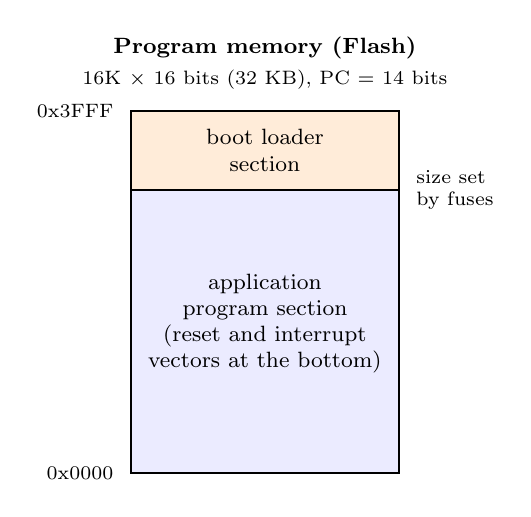
\begin{tikzpicture}[font=\small]
% Flash
\node[font=\footnotesize\bfseries] at (1.7,5.4) {Program memory (Flash)};
\node[font=\scriptsize] at (1.7,5.0) {16K $\times$ 16 bits (32 KB), PC = 14 bits};
\draw[thick,fill=blue!8] (0,0) rectangle (3.4,4.6);
\draw[thick,fill=orange!15] (0,3.6) rectangle (3.4,4.6);
\node[font=\footnotesize,align=center] at (1.7,4.1) {boot loader\\section};
\node[font=\footnotesize,align=center] at (1.7,1.9) {application\\program section\\(reset and interrupt\\vectors at the bottom)};
\node[font=\scriptsize,anchor=east] at (-0.1,0) {0x0000};
\node[font=\scriptsize,anchor=east] at (-0.1,4.6) {0x3FFF};
\node[font=\scriptsize,anchor=west,align=left] at (3.5,3.6) {size set\\by fuses};
\end{tikzpicture}
\end{document}
